% 
% Annual Cognitive Science Conference
% Sample LaTeX Paper -- Proceedings Format
% 

% Original : Ashwin Ram (ashwin@cc.gatech.edu)       04/01/1994
% Modified : Johanna Moore (jmoore@cs.pitt.edu)      03/17/1995
% Modified : David Noelle (noelle@ucsd.edu)          03/15/1996
% Modified : Pat Langley (langley@cs.stanford.edu)   01/26/1997
% Latex2e corrections by Ramin Charles Nakisa        01/28/1997 
% Modified : Tina Eliassi-Rad (eliassi@cs.wisc.edu)  01/31/1998
% Modified : Trisha Yannuzzi (trisha@ircs.upenn.edu) 12/28/1999 (in process)
% Modified : Mary Ellen Foster (M.E.Foster@ed.ac.uk) 12/11/2000
% Modified : Ken Forbus                              01/23/2004
% Modified : Eli M. Silk (esilk@pitt.edu)            05/24/2005
% Modified : Niels Taatgen (taatgen@cmu.edu)         10/24/2006
% Modified : David Noelle (dnoelle@ucmerced.edu)     11/19/2014

%% Change "letterpaper" in the following line to "a4paper" if you must.

\documentclass[10pt,letterpaper]{article}

\usepackage{cogsci}
\usepackage{pslatex}
\usepackage{apacite}

% our packages
% ---------------------------------------------------------
% \usepackage{hyperref}       % hyperlinks
% \usepackage{url}            % simple URL typesetting
\usepackage{subcaption}
\usepackage{amsmath,amsfonts,amsthm,amssymb,amsopn,bm}
\newcommand{\vct}[1]{\boldsymbol{#1}} % vector
\newcommand{\mat}[1]{\boldsymbol{#1}} % matrix

\usepackage{graphicx}
\graphicspath{{../graphs/}}
% ----------------------------------------------------------


\title{Comparing Alternative Computational Models of the Stroop Task \\Using of Effective Connectivity Analysis of fMRI Data}
 
\author{{\large \bf Micah Ketola (ketolm@uw.edu)} \\
  Department of Psychology, \\
  University of Washington, Seattle, WA 98195 USA
  \AND {\large \bf Linxing Preston Jiang (prestonj@cs.washington.edu)} \\
  Paul G. Allen School of Computer Science and Engineering\\
  University of Washington, Seattle, WA 98195 USA 
  \AND {\large \bf Andrea Stocco (stocco@uw.edu)} \\
  Department of Psychology and Institute for Learning and Brain Sciences (I-LABS), Campus Box 351525, \\
  University of Washington, Seattle, WA 98195 USA}


\begin{document}

\maketitle


\begin{abstract}
Methodological advances have made it possible to generate fMRI predictions for cognitive architectures, such as ACT-R, thus expanding the range of model predictions and making it possible to distinguish between alternative models that produce otherwise identical behavioral patterns. However, for tasks associated with relatively brief response times, fMRI predictions are often not sufficient to compare alternative models. In this paper, we outline a method based on {\it effective connectivity}, which significantly augments the amount of information that can be extracted from fMRI data to distinguish between models. We show the application of this method in the case of two competing ACT-R models of the Stroop task. Although the models make, predictably, identical behavioral and BOLD time-course predictions, patterns of functional connectivity favor one model over the other. Finally, we show that the same data suggests directions in which both models should be revised.

\textbf{Keywords:} 
ACT-R, Dynamic Causal Modeling, Cognitive Science
\end{abstract}

\section{Introduction}

One of the traditional problems in the field of cognitive modeling is deciding which of two models is right \cite{Pitt2006}. Traditionally, the most common approach has been to compare models using null-hypothesis testing procedures. In essence, conditions are identified in which the two models make qualitatively different predictions, and the hypothesized pattern is tested using classical techniques. While more sophisticated approaches have been proposed \cite{Pitt2006, Veksler2015}, this approach remains the {\it de facto} standard of the field.

The search for conditions in which two models differ is sometimes strenuous. The same behavior can occasionally be obtained through different possible internal processes and model parameters. By shedding light on more direct correlates of cognitive processes, neuroimaging data provides a potential way to distinguish between otherwise behaviorally identical results \cite{Sohn2004}. For this reason, procedures have been devised to derive neuroimaging predictions from computational models, most commonly in the domain of fMRI (\cite{Anderson2008}).

While the use of fMRI has greatly expanded upon the possible predictions that can distinguish between the two models, a number of limitations still exist. The main limitation arises from poor temporal resolution of fMRI.  However, even methods that offer a more precise temporal resolution, such as EEG or MEG, suffer from other drawbacks. For example, models often rely on specific, crucial assumptions about the order of mental steps to draw causal relationships between different modules.

Recently, \citeA{rice2019role} proposed using Transcranial Magnetic Stimulation (TMS) as a different way to test model predictions. TMS provides a way to causally interfere with specific cortical computations, thus providing both causal interference with the necessary spatio-temporal resolution. It should be noted, however, that their paper did not use this technique to compare models. 

In this paper, we describe and demonstrate an alternative and novel way to test models using neuroimaging data that addresses these concerns. This method is based on patterns of {\it effective connectivity} between brain regions. Effective connectivity is an umbrella term to characterize the functional exchange of information between two brain regions, based on the analysis of their respective time series. Because effective connectivity provides measures of directional communication between two regions, it can be used to examine the internal dynamics of a computational model.  Furthermore, because effective connectivity can be estimated from fMRI or EEG data, it expands the dimensions across which models can be compared without requiring collecting additional data.

In the remainder of this paper, we will outline our method and apply it to a specific, and exquisitely cognitive case, namely, determining which of two prominent computational explanations for the Stroop interference best explains the data.    

\subsection{ACT-R}

Although our method could be applied to any computational model, for convenience, it will be demonstrated with two models developed in the Adaptive Control of Thought--Rational (ACT-R) cognitive architecture \cite{Anderson2004}. This choice was made for three reasons.  First, ACT-R is the most successful and widespread architecture, having been used in hundreds of publications since its inception, and by far the most popular in the field of cognitive research \cite{Kotseruba2018}; Thus, it provides an excellent domain in which to demonstrate the procedure. Second, ACT-R already provides well-tested mappings between architectural components and brain regions with established procedures to predict fMRI activity from model simulations. Therefore, these assumptions can be adopted without the need to provide additional justifications. Finally, the assumptions of ACT-R provide a reasonable mechanism to translate model activity into effective connectivity. As it will be shown, this is based on the functional requirements of the procedural module, which have been examined and discussed in the past.

ACT-R represents knowledge in two formats, declarative and procedural. Declarative knowledge is made of record-like structures, called {\it chunks}, which capture semantic memories (“Paris is the capital of France”), perceptual inputs (“A black triangle is on the screen”), and motor commands (“Press the spacebar”). Procedural knowledge consists of production rules (or simply ``productions''), state-action pairs that encode the specific policy to perform a task. In summary, chunks represent information, and productions act upon them.

Chunks are processed by functionally specialized modules. For instance, perceptual modules create new chunks to represent the contents of the outside world, and a memory module maintains chunks in long-term memory. Each module contains one or more buffers, limited-capacity stores that contain at most one chunk. Buffers are the only mechanisms through which chunks and productions interact: Chunks can be inspected, copied, and modified by productions when exposed into buffers. 

As noted above, much work has been dedicated to map ACT-R modules to corresponding neural circuits. This work has yielded a number of reliable functional mappings, including the association between anterior cingulate cortex and the goal buffer in the goal module \cite{fincham2006distinct,sohn2007anticipation}, between the lateral prefrontal cortex and the retrieval buffer of the long-term memory module \cite{fincham2006distinct,danker2008rational}, between posterior parietal cortex and the imaginal buffer of working memory (Anderson, 2005; Anderson, Albert, et al., 2005; Borst et al., 2010; Sohn, Ursu, Anderson, Stenger, & Carter, 2000), between the fusiform gyrus and the visual buffer in the visual module (Anderson, 2005; 2007), and between the primary motor cortex and the manual buffer in the motor module (Anderson, 2005; Anderson et al., 2004).



\subsection{Dynamic Causal Modeling}

To estimate effective connectivity, we adopted a framework known as Dynamic Causal Modeling (DCM) \cite{Friston2003, Stocco2018}. In essence, DCM is procedure to model the time-course of in brain activity in a set of brain regions through a dynamical system of other brain regions and event vectors. Specifically, the time course of activity of a region $i$ is expressed as a bilinear state equation:

\begin{equation}
\dot{\vct{y}} = \mat{A}\vct{y} + \sum_{i}x_i\mat{B}(i)\vct{y} + \mat{C}\vct{x}
\label{DCMEquation}
\end{equation}

where $\mat{A}$ defines intrinsic connectivity between different regions (fixed connectivity), $\mat{C}$ defines effects by task inputs, and $\mat{B}$ defines the modular effects that task conditions have on the connectivity between regions (modulation of connectivity). %The overall ``effect'' of one task condition to another was then approximated by the element-wise product of $\mat{A}$ and $\mat{B}$, namely

Effective connectivity can be thought of as a way to measure to degree of directional information transfer between Regions of Interest (ROIs).

%\[\text{effective connectivity} = \mat{A} \odot \mat{B}\]

\subsection{ACT-R Predictions for Effective Connectivity }

Because effective connectivity can be interpreted as information transfer, a direct link can be made between this measure and the nature of ACT-R computations. As shown above, ACT-R works by firing one production at a time during its cognitive cycle; this production, in turn, changes the state of the system by modifying or copying information from one buffer to the other. For example, in what is perhaps the most common operation in ACT-R models, a production rule extracts values from the slots of chunks placed in either the imaginal or the visual buffer (to extract contextual task information) and places them in the retrieval buffer, so that they function as constraints for memory retrieval.  

The idea that variables in production rules can be used as proxy of effective connectivity is not entirely new. It was initially suggested in Anderson et al., 2008, in which the authors speculated that common functional connectivity patterns in the brain reflect the ubiquity of common operations that link different buffers---such as the production described.

The idea ran against established identification between the procedural module and the basal ganglia (Anderson,2005). However, it has been noted before that the function of the basal ganglia is to direct inputs to cortical regions, a role that is both compatible with the procedural module and with the proposed interpretation of effective connectivity.

To operationalize this definition, we followed a simple procedure. First, an $N \times N$ squared matrix ${\mat{E}}$, with $N$ being the number of buffers examined, is generated and initialized to zeros. Then, the target model is run and its trace is segmented into epochs of interest  (e.g., all the trials of the same conditions). The structure of each production rule firing within that epoch is then examined. For each variable in the production rule, the {\it source} buffer $S$ at which the variable is introduced (or, technically, bound to a value) in the left-hand side and the {\it target} buffer $T$ in which the bound value is placed are recorded. The value of the matrix cell $\mat{E}_{S,T}$ is then incremented by one. If a variable appears in multiple source buffers $S_1, S_2 \dots S_L$ or target buffers $T_1, T_2 \dots T_L$, then all the cells $\mat{E}_{i \in K, j \in  L}$ are updated. When all the productions have been examined, $\mat{E}$ is taken to represent the predicted effective connectivity for that particular condition. 

%Since each trial the Stroop task is generally performed within one second, it is expected that the three information processing modules: imaginal, goal, and retrieval should have strong correlations since their activation could only be captured in one image scan given our sampling rate $TR = 1.5$ seconds. Furthermore, if the imaginal module is for intermediate information processing as ACT-R suggests, an increasing connectivity effect from imaginal module to goal module (``problem state'') is expected in order to process the unmatching color and text semantics in incongruent trials.

\section{An Application of the Method: \\ ACT-R Models of the Stroop Task}

To demonstrate this method, two models of the Stroop task were implemented. They were derived from previously proposed alternative models of the Stroop task, authored by Marsha Lovett \cite{Lovett2005} and by Erik Altmann \cite{VanMaanen2009}. Since both models were published before ACT-R was modified to account for neuroimaging data, they were re-implemented in the most recent version of ACT-R (version 7.6). This reimplementation processes also ensured that the two models interacted with the task using the same sensorimotor mechanisms, i.e. visual objects and responses were given in the same way. From now on, we will refer to these two models as the Altmann-like model and the Lovett-like model. 

The re-implemented models maintained the underlying assumptions of their original versions. Specifically, the two models provide different explanations about the nature of Stroop interference. In the Altmann model (Figure 3A), Stroop interference is driven by interference at the lemma layer. When a word is processed, it has direct access to its' lemma, or conceptual representation. Access to the lemma of a color is indirect, requiring an extra retrieval not seen with words. The model assumes that the word dimension of the Stroop stimulus is automatically processed first, therefore activating the lemma attached to the word dimension of the stimulus. As it tries to process the color dimension of the stimulus, the word-lemma is active and can either facilitate or inhibit retrieval of the correct color-lemma. In cases of facilitation, activation from the word-lemma spreads to the coinciding color-lemma, increasing the likelihood of correct retrieval on congruent trials. Oppositely, on incongruent trials, this activation spreads to the incorrect color-lemma, creating increased competition between color-lemmas and introducing ambiguity. For neutral trials, the word-lemma has no corresponding color-lemma, resulting in neither facilitation nor inhibition. The color-lemma is compared to visual cues and re-selected if inconsistent or otherwise used in further processing. A manual response is then retrieved using the color-lemma, and used to press a key on the keyboard. 

\begin{figure}[ht]
\centering
  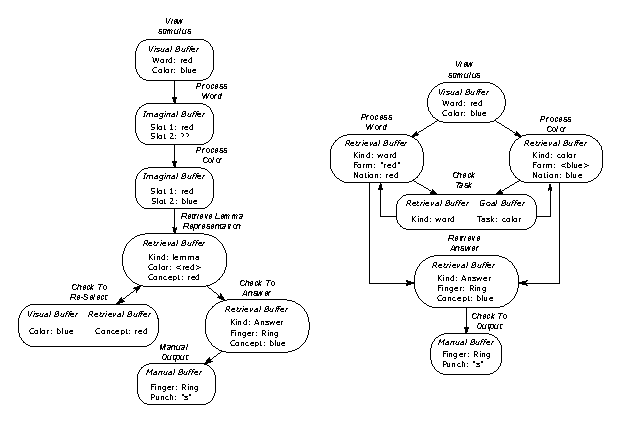
\includegraphics[width=\linewidth]{both_models.eps}
  \caption{Flow-chart representation of the strategies used by the Altmann model (``A'', left) and the Lovett model (``B'', right) when processing Stroop trials.}
\end{figure}%


In the Lovett model (Figure 3B), Stroop interference is driven by the competition between alternative \textit{word-association chunks}, linking a word to its' conceptual representation, and \textit{color-association chunks}, linking a color to its' conceptual representation. The idea is similar to lemmas from the Altmann model, but in this case both types of dimension-associated chunks need to be retrieved. The Lovett model accounts for individual differences by supporting various strategies to complete the task. In contrast to the Altmann model, this model allows for processing of either stimulus dimension first, but is highly biased towards the word dimension. From either path, chunks associated with the processed dimension are retrieved. Processing can maintain with the retrieval of an answer directly, or the task is checked. Answering directly allows for incorrect answers on incongruent trials and fast responses on congruent trials. When the task is checked, the model compares the dimension of the processed chunk to the goal, which for our purpose is to always respond according to the color of the stimulus. If there is a mismatch, processing continues with the alternative stimulus dimension. Now when retrieving the alternative dimension-associated chunk, the previously retrieved chunk has the same effect as in the Altmann model, facilitating retrieval on congruent trials, having no effect on neutral trials, and inhibiting retrieval on incongruent trials. Notably, this does not necessarily happen on every trial, as there are alternate pathways and strategies, and the model will not retrieve the wrong answer at this point. The base-level activations are set in such a way that incongruent chunks slow retrieval of the correct chunk, and congruent chunks facilitate retrieval of the correct chunk. Once the correct dimension-associated chunk is retrieved, a manual answer is retrieved using the matching chunk, and used to press a key on the keyboard. 

The two models offer an ideal comparison for two reasons. First, they deal with an experimental paradigm that is representative of research in cognitive neuroscience. Second, they embody different and opposing views about the nature of Stroop interference. Most importantly, these two models exemplify the limits of ACT-R's predictive capacity in neuroimaging. The two models, in fact, make use of the same five buffers (visual, motor, goal, imaginal, retrieval) and produce indistinguishable BOLD responses. The latter is a consequence of the difference between the resolution of the BOLD responses recorded in fMRI, which is much more sluggish and spans multiple seconds, and the time course of a Stroop trial, which is typically on the order of a few hundred milliseconds. When considering that time needed for perceptual and visual processes (identical in the two models), the difference between the two models is concentrated in a 300 ms window in which different interactions between imaginal, goal, and retrieval buffers are posited.

Crucially, although these different interactions produce indistinguishable BOLD traces, they do produce different effective connectivity matrices.

%Traditionally, hemodynamic response functions (HRFs) are convolved with the event matrix (i.e., information processing of each module) derived from ACT-R to simulate fMRI data for various tasks \cite{Anderson2004,Lindquist2009}. A common choice of HRF, the double gamma function, is define as 
%\[f(t, \alpha, \beta) = \frac{t^{\alpha - 1}e^{-\beta t}}{\Gamma(\alpha)}\]
%where $t$ is time, $\alpha$ and $\beta$ define the scale and shape of the function, respectively, and $\Gamma(x) = (x - 1)!$ for $x \in \mathbf{R}$ \cite{Poldrack, Cignetti2016}. Then the simulated data is visually compared to the real fMRI data to check for similarities, or simple metrics such as mean square error are applied \cite{Anderson2004, Borst2017}. More rigorous analysis without the assumption of brain activations being HRF-shaped could be useful to verify ACT-R in a bottom-up approach. In this project, both brain connectivity analysis and mixture models are proposed to discover meaningful structures directly from the data with few assumptions. Specifically, covariance estimation and dynamic causal modeling were used to study brain region connectivity, and Gaussian Mixture Models were used to estimate the distributions of individual brain activation in each module.

\section{Materials and Methods}

\subsection{Experimental Dataset}

In this analysis, we used fMRI publicly available from on an open repository\footnote{The data is available on OpenNeuro at the following URL:  https://openneuro.org/datasets/ds000164/versions/00001}. The original data was collected at Carnegie Mellon University by Timothy Verstynen, and published in Verstynen et al. \cite{Verstynen2014}.

\subsection{Participants}

The dataset contained data from $N=30$ participants (10 female), aged 21--45 (mean 31). The recruitment  procedures can be found in the original publication \cite{Verstynen2014}.

\subsection{Experimental Task}

Participants performed a manual-response version of the Stroop task \cite{Stroop1935}, during which the subjects were asked to indicate the color of a written word presented in the center of the screen. The responses 

\subsection{Image Acquisition and Preprocessing}

As described in \citeA{Verstynen2014}, the original raw data was acquired using a Siemens 
For the purpose of our analysis, the original raw data was re-processed using a different pipeline than the one indicated in the original publication. Specifically, the data were analyzed using SPM12 (Wellcome Department of Imaging Neuroscience, www.fil.ion.ucl.ac.uk/spm). Images were corrected for differences in slice acquisition time, spatially realigned to the first image in the series, normalized to the Montreal Neurological Institute (MNI) ICBM 152 template, resampled to 2 × 2 × 2 mm voxels, and finally smoothed with a 8 × 8 × 8-mm full-width-at-half-maximum Gaussian kernel to decrease spatial noise and to accommodate individual differences in anatomy. %Statistical analyses were performed on individual and group data using the general linear model, as implemented in SPM8 (Friston, Ashburner, Kiebel, Nichols, and Penny, 2006). For individual participants, fixed-effects models that incorporated a high-pass filter with a cutoff of 128 s and an AR(1) correction for serial autocorrelation were used to estimate parameters. The models included one regressor for the response and one regressor for each of the four experimental conditions (novel instructions, practiced instructions, execution of novel instructions, and execution of practiced instructions). 

\subsection{Regions of Interest}

DCM analysis is performed on fMRI time-series extracted from specific ROIs. In our case, the ROIs correspond to the specific brain regions that have been previously identified as corresponding to ACT-R buffers. Module-specific BOLD time series were extracted for each  The Talairach coordinates used for each module in the brain followed the convention used by \cite{Anderson2008, Borst2017}. The algorithms described in \cite{Lacadie2008} were used to convert Talairach coordinates to Montreal Neurological Imaging Institute (MNI) coordinates. The ROI mask files were created through FSL \cite{Woolrich2009} of size 16 mm (125 voxels in total) then used to extract fMRI time series from each voxel in each ROI. Principal Component Analysis was then applied on all the extracted time series to identify the time series that best characterized each ROI. The largest principle component was used to project the original data to the new space with more than 75\% of the variance explained in each module. 

\subsection{Dynamic Causal Modeling Analysis}

Because DCM is a model-based technique, estimates of connectivity can only derived from parameters corresponding to the specified connectivity between ROIs.  To gather complete estimates of connectivity, an unconstrained, fully connected model was generated, in which any ROI was bidirectionally connected to all the others. Furthermore, to identify different patterns of connectivity between conditions, both matrices $B$ and $C$ were used. Specifically, matrix $C$ was used to specify the onset and offset of stimuli, and drive the activity  of the ``visual'' ROI, thus initiating trial-specific activity in the network. In addition, we used the modulatory matrix $B$ to specify modulatory effects of condition-specific trials (congruent, neutral, and incongruent) and the ROI connectivity parameters $\mat{A}$. Thus, the effective connectivity matrix $E_k$ specific to task condition $k$ can be expressed as the element-wise product of $\mat{A}$ and the modulatory effects of condition $k$ $\mat{B}_k$, namely:

\begin{equation}
\mat{E}_k = \mat{A} + \mat{A} \odot \mat{B}_k
\label{dcm:trick}
\end{equation}

As it is common in DCM, all the parameters were identified using a Expectation-Maximization procedure over a probability distribution of parameter value. 

 
\section{Result}

Figure~\ref{fig:conn} shows the connectivity analysis results between modules. Figure~\ref{fig:conn} (a) shows the functional connectivity between retrieval and imaginal is high as expected, while that between imaginal and goal is not as high. (b) and (c) show the results of DCM in both congruent and incongruent trials averaged across subjects through Bayesian parameter averaging \cite{Kasess2010} (see Appendix C), and (d) shows the difference in the effective connectivity in different tasks (incongruent - congruent). Circled parts in (d) confirm the effect we expect from ACT-R: in incongruent trials, there is a significant increase between imaginal and goal modules to account for the unmatching color and semantic condition. More importantly, their effect on the output (i.e., the manual module) also changes drastically. Compared to congruent trials, there is a significant decrease effect from goal to manual and a significant increase effect from imaginal to manual, suggesting that information about the final decision is delivered by imaginal rather than goal in incongruent trials. Again, this supports ACT-R's assumption that little imaginal involvement is needed in congruent trials. 

\section{Discussion}

This paper has shown how analysis of effective connectivity can be used to supplement traditional, GLM-based analysis of neuroimaging data in distinguishing between alternative models. While effective connectivity analysis has been used in cognitive neuroscience for more than a decade, this is the first time, to the best of our knowledge, that this method is used in conjunction with a cognitive modeling approach, and with cognitive architectures in particular.

In outlining our method, we made the specific choice of using ACT-R as a modeling paradigm and DCM as a technique to estimate effective connectivity. Neither of these choices, however, are absolute requirements. Connectivity estimates can be gathered from many types of models; the procedure described in this paper certainly applies to other production system-based architecture, like Soar and EPIC, as well. Similarly, although connectivity was estimated with DCM,  other methods could be possibly used. For example, Granger Causality. %We prefered DCM because it made it easier to estimate condition-specific Notice that, however, Granger causality could be difficult to apply estimating condition-specific effects, since each trial corresponds to one or two time points at the fMRI resolution. By contrast, in DCM it was trivial to solve the problem using the solution in Equation \ref{dcm:trick}.

It is interesting to note that DCM could be used in alternative different ways. For example, instead of extracting data using DCM, the patterns of connectivity identified for the two models could be translated into corresponding DCM models, and the two models could be compared in terms of data fit, using any of the techniques that have been proposed. The solution outlined here, however, is in principle more general.

Although we have demonstrated that effective connectivity can be used to compare model, it is worth noting that the connectivity matrices obtained from the data can be used to inform model development as well. It is apparent that neither the Lovett nor the Altmann model provide good fits to the data. By comparing their predicted connectivity matrices against the empirical ones, some patterns can be noted. Because the differences correspond to variables in production rules, the comparison suggests which other. In theory, and provided reasonable task constraints, an analysis of the effective connectivity matrices might be used to automatically generate production rules that would match the data. We see this an exciting opportunity for future research.

That's an exciting possibility for the future.

\section{Formalities, Footnotes, and Floats}

Use standard APA citation format. Citations within the text should
include the author's last name and year. If the authors' names are
included in the sentence, place only the year in parentheses, as in
\citeA{NewellSimon1972a}, but otherwise place the entire reference in
parentheses with the authors and year separated by a comma
\cite{NewellSimon1972a}. List multiple references alphabetically and
separate them by semicolons
\cite{ChalnickBillman1988a,NewellSimon1972a}. Use the
``et~al.'' construction only after listing all the authors to a
publication in an earlier reference and for citations with four or
more authors.


\subsection{Tables}

Number tables consecutively. Table~\ref{sample-table}. You may float
tables to the top or bottom of a column, or set wide tables across
both columns.

 	\begin{table}[!ht]
\begin{center} 
\caption{Sample table title.} 
\label{sample-table} 
\vskip 0.12in
\begin{tabular}{ll} 
\hline
Error type    &  Example \\
\hline
Take smaller        &   63 - 44 = 21 \\
Always borrow~~~~   &   96 - 42 = 34 \\
0 - N = N           &   70 - 47 = 37 \\
0 - N = 0           &   70 - 47 = 30 \\
\hline
\end{tabular} 
\end{center} 
\end{table}

%\begin{figure}[ht]
%\centering
  %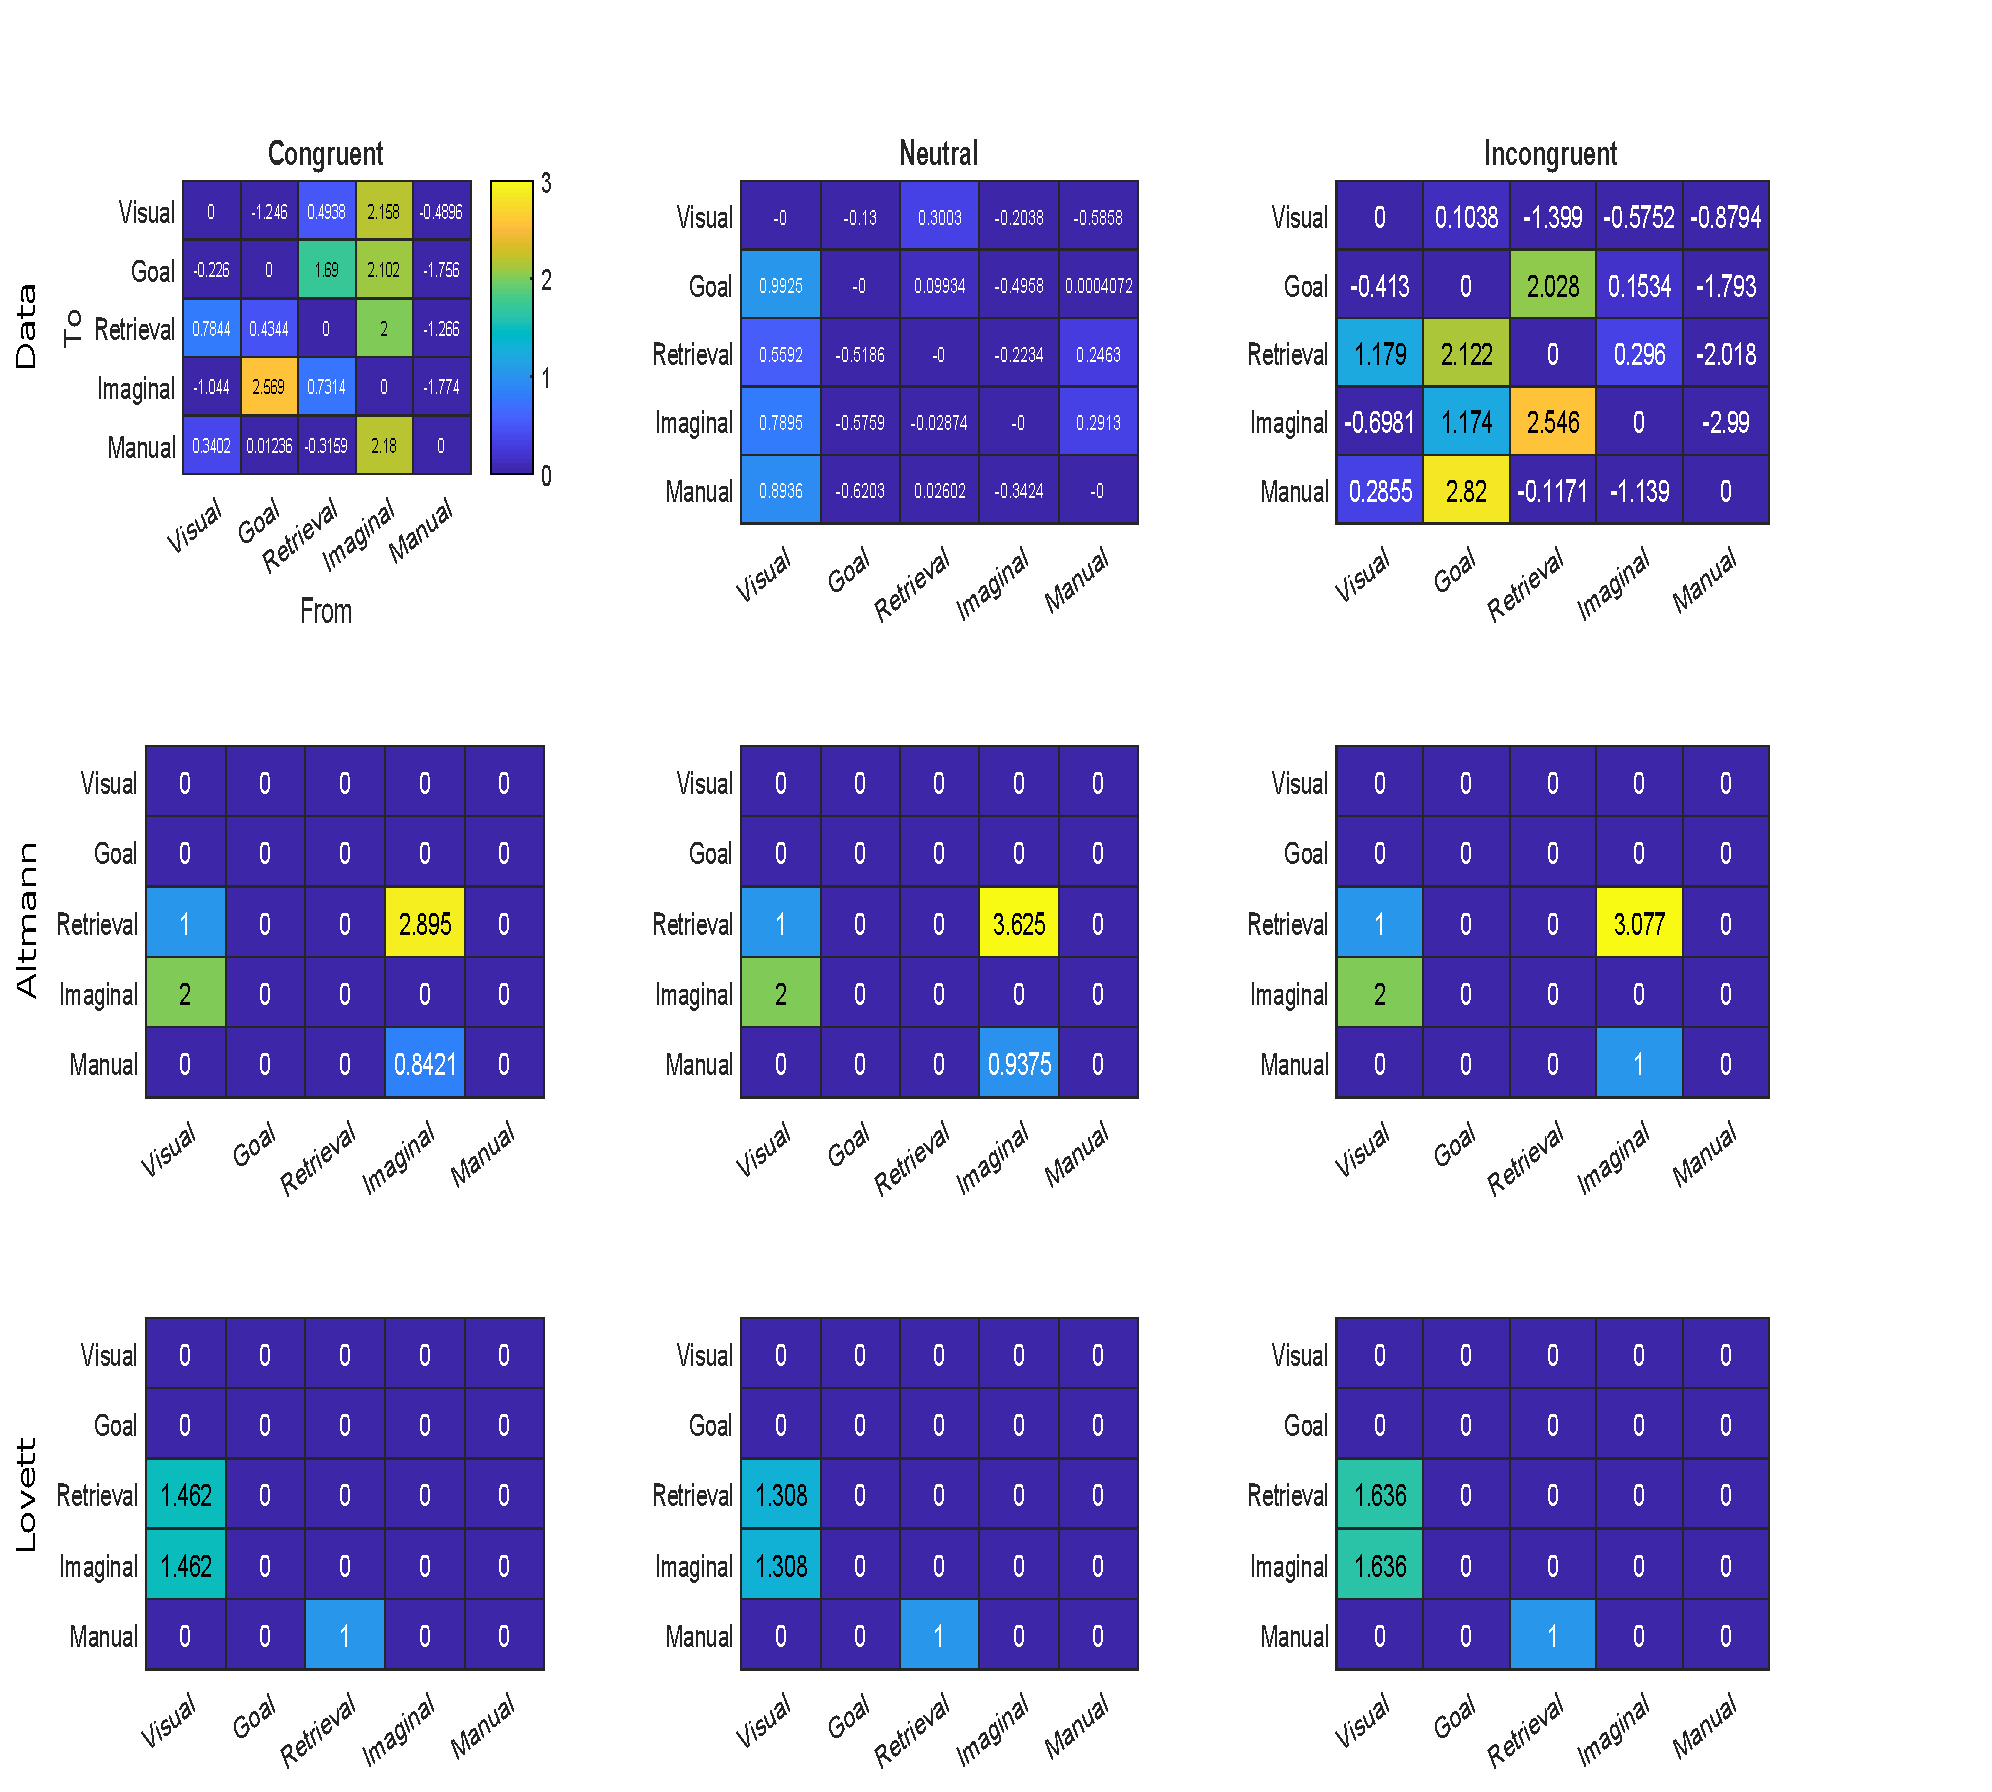
\includegraphics[width=\linewidth]{9x9.eps}
  %\caption{9x9.}
%\end{figure}%

\begin{figure}[ht]
\centering
\begin{subfigure}{.11\textwidth}
  \centering
  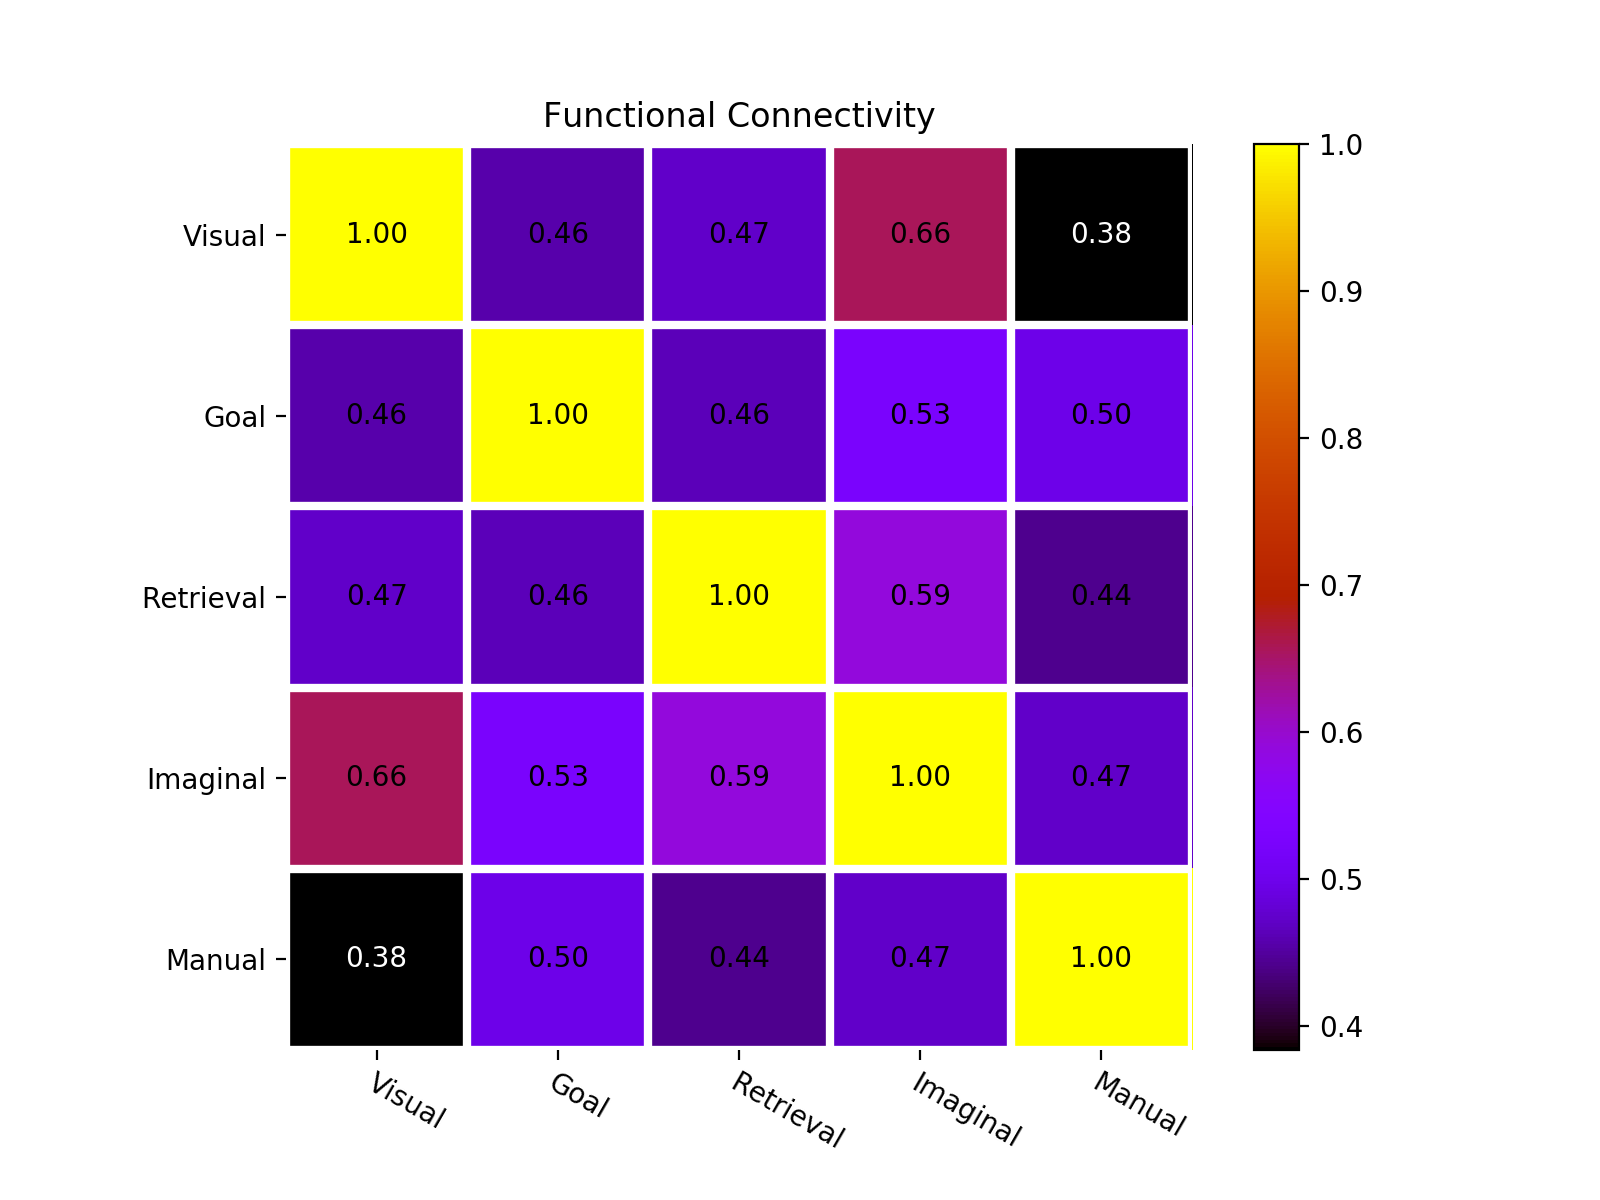
\includegraphics[width=\linewidth]{func_conn.png}
  \caption{}
\end{subfigure}%
\begin{subfigure}{.11\textwidth}
  \centering
  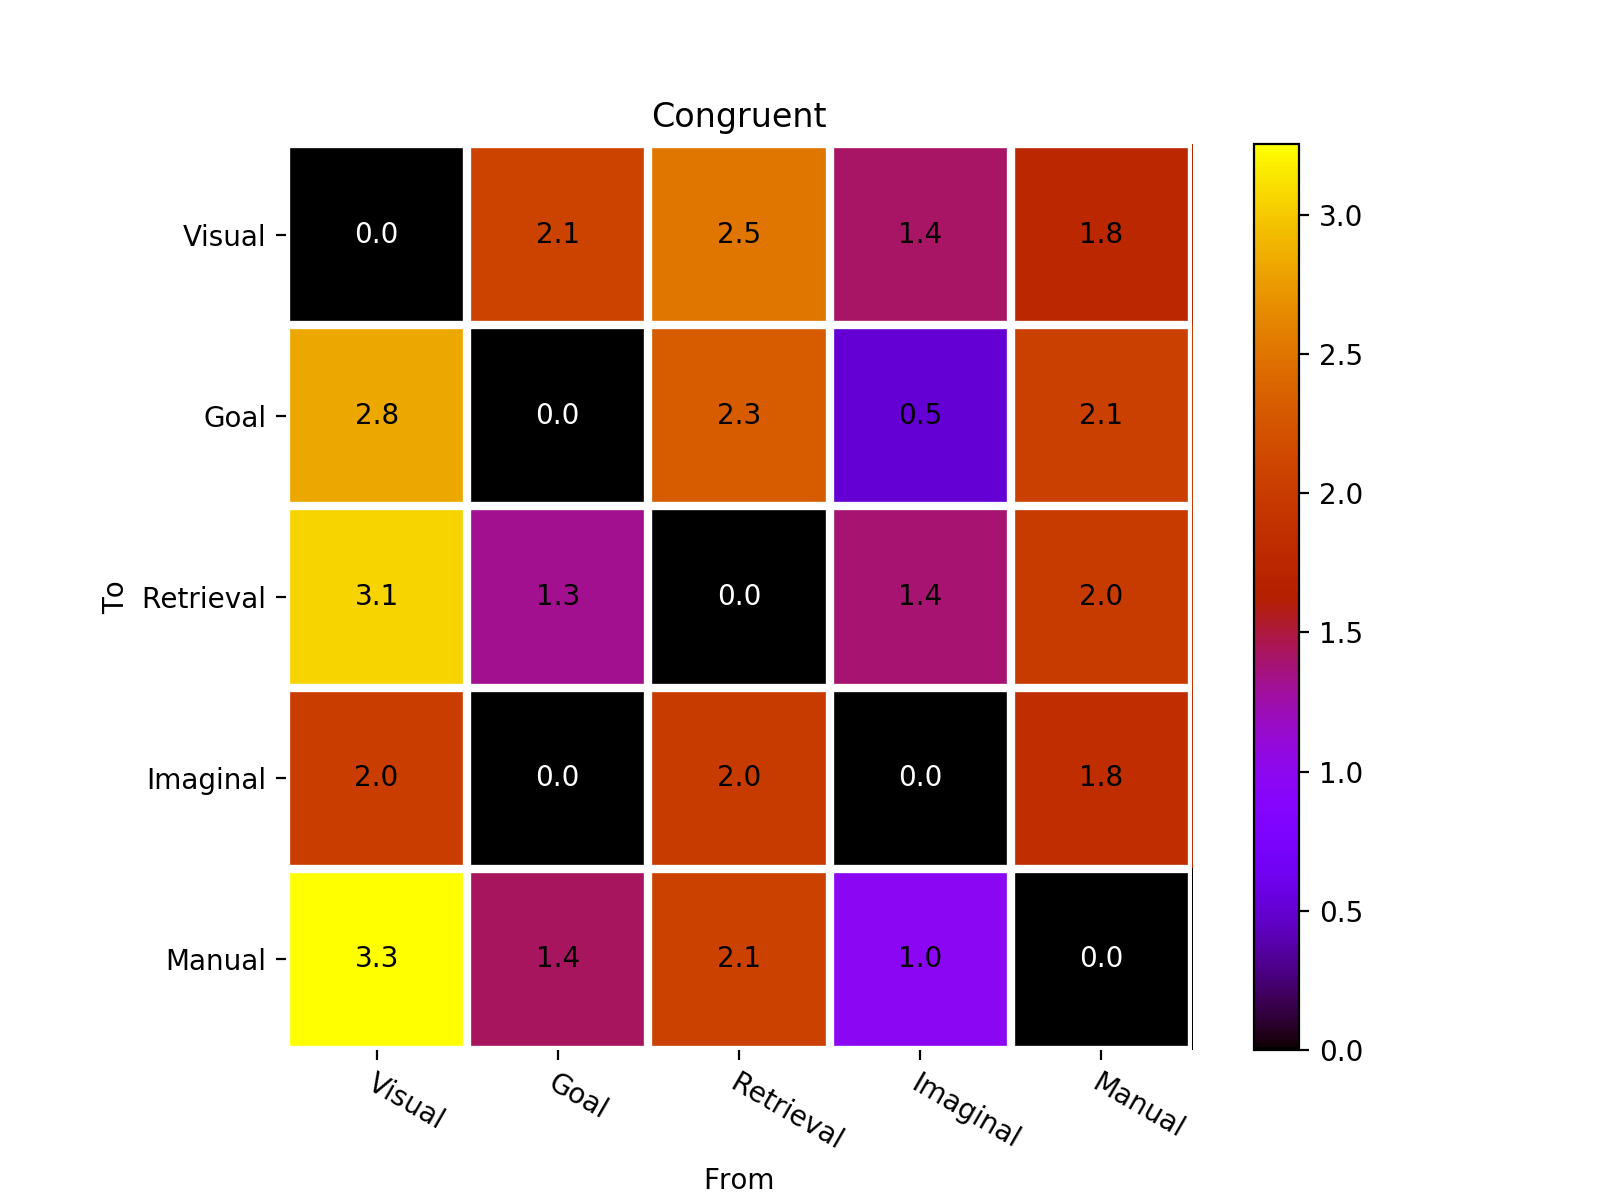
\includegraphics[width=\linewidth]{Congruent_effect_conn.png}
  \caption{}
\end{subfigure}
\begin{subfigure}{.11\textwidth}
  \centering
  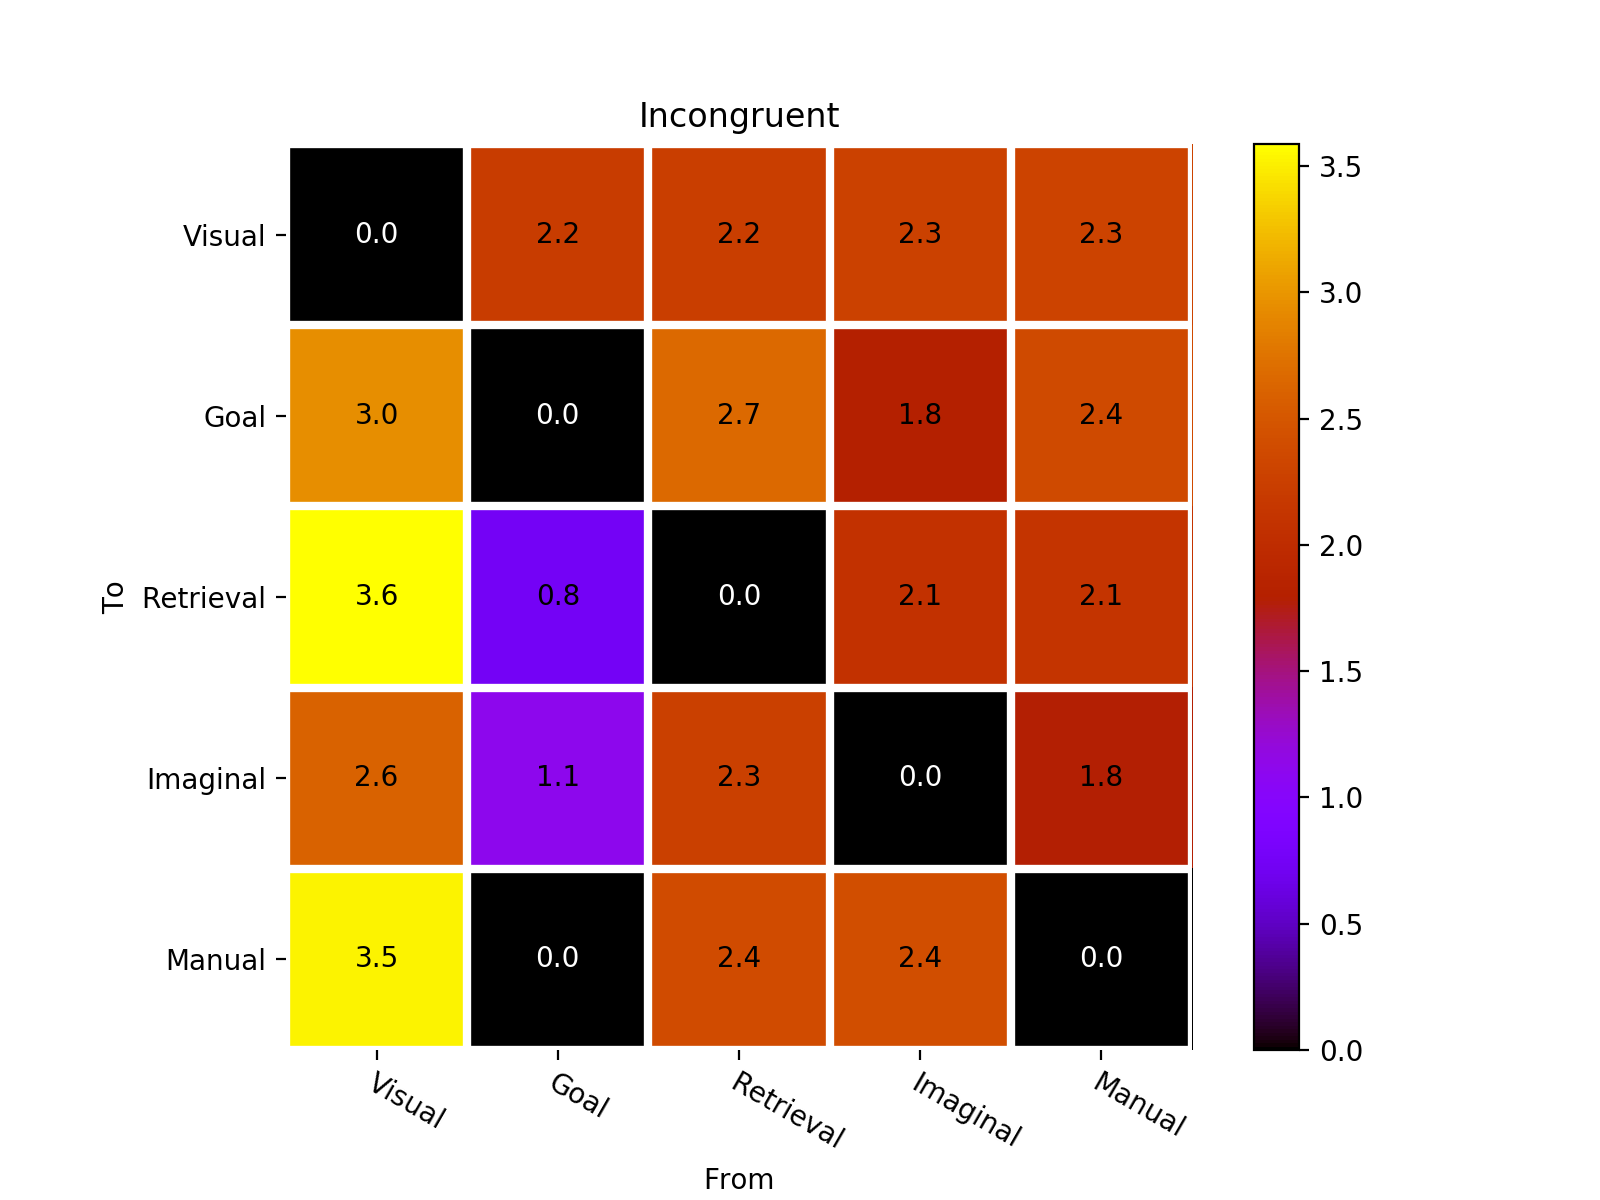
\includegraphics[width=\linewidth]{Incongruent_effect_conn.png}
  \caption{}
\end{subfigure}%
\caption{Brain region connectivity results: (a) Functional connectivity analysis shows strong brain signal activation between imaginal and retrieval, but not imaginal and goal; (b) Effective connectivity in congruent trials: similar strong effects between retrieval and imaginal are shown (data is zero-min) ; (c) Effective connectivity in incongruent trials: increasing connectivity between imaginal and goal are shown (data is zero-min); (d) Difference of effective connectivity in different tasks (incongruent - congruent): circled regions show brain connectivity dynamics in different tasks.}
\label{fig:conn}
\end{figure}


\section{Acknowledgments}

Place acknowledgments (including funding information) in a section at
the end of the paper.


\bibliographystyle{apacite}
\setlength{\bibleftmargin}{.125in}
\setlength{\bibindent}{-\bibleftmargin}
\bibliography{ref}


\end{document}
